\question (南京理工大学,2001年)无向图G=(V,E),其中V=\{a,b,c,d,e,f\},E=\{(a,b),(a,e),(a,c),(b,e),(c,f),(f,d),(e,d)\},对该图进行深度优先遍历,得到的顶点序列正确的是(
)
\par\twoch{a,b,e,c,d,f}{a,c,f,e,b,d}{a,e,b,c,f,d}{\textcolor{red}{a,e,d,f,c,b}}
\begin{solution}先画出下图,再依次套用各个选项的顶点次序。A选项,abe后面应该是d,排除;B选项,acf后面应该是d,排除;C选项,ae后面应该是d,排除;D选项,aedfcb为可能得到的顶点序列。
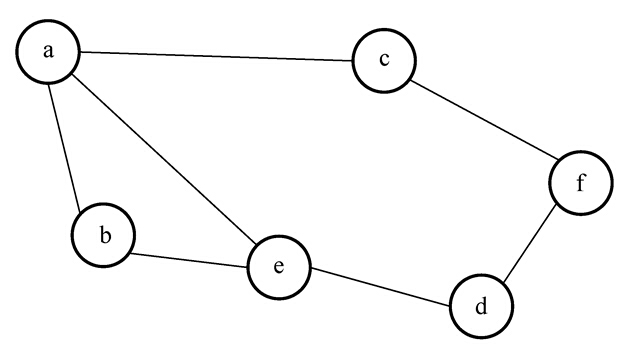
\includegraphics[width=2.08333in,height=2.08333in]{computerassets/cc2b9294e0c91ea82d13cd032d0b3342.jpeg}
\end{solution}
\question (北京交通大学,2005年)已知一个有向图如下图所示,则从顶点a出发进行深度优先遍历,不可能得到的DFS序列为(
)
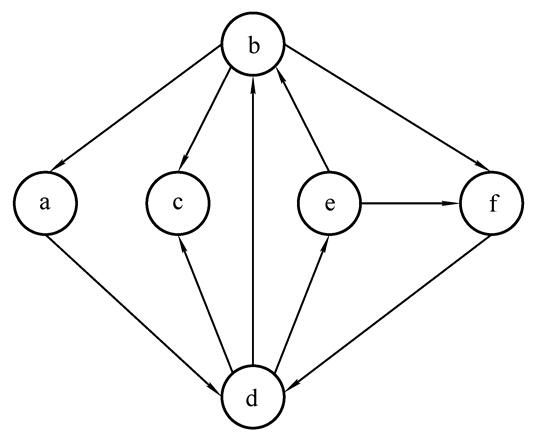
\includegraphics[width=3.12500in,height=2.57292in]{computerassets/b49915e01029e13a40983c900a23f874.jpeg}
\par\twoch{\textcolor{red}{adbefc}}{adcefb}{adcbfe}{adefbc}
\begin{solution}A项在遍历到结点b时,没有服从深度优先继续遍历c或者f,违背了DFS算法的原则,因此是不可能得到的DFS序列。其他选项均满足DFS算法的原则。
\end{solution}
\question (中山大学,2006年)若一个n个结点和e条边的图采用邻接表作为其存储结构,其深度优先遍历的时间复杂度为(
)
\par\fourch{}{}{\textcolor{red}{}}{}
\begin{solution}深度优先遍历需要访问一遍邻接表结点(包括头结点),则时间复杂度即为O(n+e)。
\end{solution}
\question (华中科技大学,2007年)采用邻接表存储的图的广度优先遍历算法类似于二叉树的(
)算法
\par\twoch{先序遍历}{中序遍历}{后序遍历}{\textcolor{red}{按层遍历}}
\begin{solution}图的广度优先类似于二叉树的层次遍历,因为都用到了队列,而先序、中序和后序均用到栈。
\end{solution}
\question (中国矿业大学,2004年)图的遍历算法BFS中用到辅助队列,每个顶点最多进队(
)次
\par\twoch{\textcolor{red}{1}}{2}{3}{不确定}
\begin{solution}由于图的BFS算法中,每个结点进队之前在其标志位上要作记录,下次遇到已作记录的结点时,就不会再将其进队,所以每个顶点最多进队一次。
\end{solution}
\question 若对如下无向图进行遍历,则下列选项中,不是广度优先遍历序列的是( ~)。
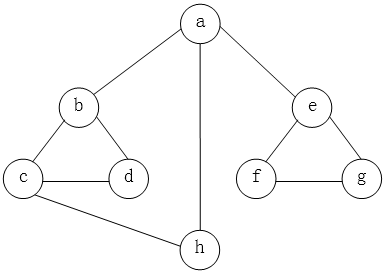
\includegraphics[width=3.33333in,height=2.36458in]{computerassets/CFE9736FE4AE21334B706E881EEACECC.png}
\par\fourch{h,c,a,b,d,e,g,f}{e,a,f,g,b,h,c,d}{d,b,c,a,h,e,f,g}{\textcolor{red}{a,b,c,d,h,e,f,g}}
\begin{solution}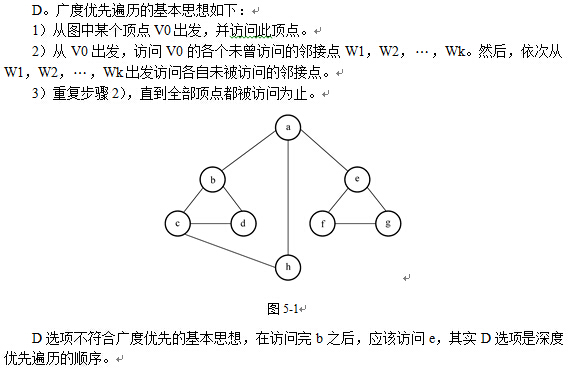
\includegraphics[width=3.33333in,height=2.16667in]{computerassets/1199b21715cba25d61384b063c453f9a.jpeg}
\end{solution}
\question (南开大学,2004年)判断有向图是否存在回路,除了可以利用拓扑排序的方法外,还可以利用(
)
\par\twoch{求关键路径的方法}{求最短路径的Dijkstra方法}{\textcolor{red}{深度优先遍历算法}}{广度优先遍历算法}
\begin{solution}对每个点标记,若深度优先访问到已标记的点则说明存在回路。
\end{solution}
\question (中山大学,2004年)下图为无向图,其从A出发的广度优先遍历结果可以为(
~)

~
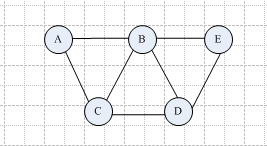
\includegraphics[width=2.78125in,height=1.52083in]{computerassets/1a724d66add415b16fa638eefae7110f.png}
\par\twoch{ABECD}{\textcolor{red}{ACBDE}}{ACDBE}{ABDEC}
\begin{solution}从A出发进行广度优先遍历,接下来两个顶点比是B和C,也就是广度优先遍历序列前3个只可能是ABC或ACB,只有答案B满足
\end{solution}
\question (南京邮电大学,2006年)下面( )算法可用于求无向图的所有连通分量
\par\twoch{\textcolor{red}{广度优先遍历}}{拓扑排序}{求最短路径}{求关键路径}
\begin{solution}从图中的一个顶点进行广度优先搜索可以将这个顶点连通的顶点全部遍历,也就找到了该顶点所在的连通分量,因此广度优先遍历可以求出无向图的所有连通分量
\end{solution}
